\documentclass[12pt,twocolumn]{IEEEtran11}

\usepackage{times}
\usepackage{epsfig}
\usepackage[T1]{fontenc}
\usepackage{graphicx}
\usepackage{subfigure}
\def\BibTeX{{\rm B\kern-.05em{\sc i\kern-.025em b}\kern-.08em
    T\kern-.1667em\lower.7ex\hbox{E}\kern-.125emX}}

\oddsidemargin -15pt
\evensidemargin -15pt
\leftmargin 0 pt
\topmargin -30pt
\textwidth = 6.9 in
\textheight = 9.0 in

\newcommand{\itembase}{\setlength{\itemsep}{0pt}}
\newcommand{\eg}{{\it e.g., }}
\newcommand{\ie}{{\it i.e., }}
\graphicspath{{FIG/}}

\begin{document}
\bibliographystyle{IEEE}

\title{\Large \bf 
Survey on Implementations and Performance of Three
Distributed File Systems
%Survey on Bottlenecks and Best Practices of Three Implementations of
%Distributed File Systems
}
\author{
Samuel Li\\
Information and Computer Science Department\\
University of Oregon\\
{\em samuelli@cs.uoregon.edu}
}
\maketitle
% You have to do this to suppress page numbers.  Don't ask.
%\pagestyle{empty}
\begin{abstract}
File systems are crucial components of supercomputers and internet-based
service providers, such as Google.
%
Often, file systems consist of many file servers
to provide capacity, performance, and reliability.
%
They are organized as a distributed system 
to provide functionalities of a file system.
%
A distributed file system can have several performance challenges,
due to the distributed nature of the file system itself,
and the high concurrency nature of the supercomputer applications.
%
This survey paper studies architecture and performance issues of three widely 
used file systems: Google File System, GPFS, and Lustre.
%
It provides the readers a better understanding of how distributed system
works, and what to expect from a distributed file system.
%
%The scope of performance issues include identificatin of bottlenecks
%and best approaches to minimize impact of these bottlenecks.
\end{abstract}

%\begin{keywords} 
%Quality Adaptive Streaming, Peer-to-Peer, Internet
%\end{keywords}

\section{Introduction}
\label{sec:intro}
File systems are a crucial component of many large-scale systems, 
namely the supercomputers and internet-based service providers.
%
While the computational capacity of modern supercomputers are keep growing,
the file system performance is not keep up the pace, in terms of both
the storage capacity and data transfer throughput.
%
Distributed file systems are widely used to tackle this problem.
%
On the one hand, distributed file systems enables a large number of commodity
storage devices to connect together and act like a unified storage space, 
which expands the storage capacity.
%
On the other hand, distributed file systems can potentially aggregate file
I/O operations from single storage devices together, providing a high
data transfer throughput. 
%
This survey paper sheds some light on the architecture as well as various
performance issues of distributed file systems.

%This survey paper identifies common performance issues in 
%the distributed file systems, 
%and explores approaches to minimize impacts of these issues.
%
This survey paper specifically looks into three popular distributed 
file systems: Google File System GPFS, and Lustre.
%
Google File System~\cite{ghemawat2003google} is designed by Google and used 
exclusively by Google.
%
GPFS~\cite{Schmuck2002,barkes1998gpfs} is a proprietary system owned by IBM, and
it also powers many supercomputers.
%
Lustre~\cite{Schwan2003} is open-sourced and powers many of the 
world's fastest supercomputers.
%
We will especially focused on three aspects of these file systems:
1) different architecture design,
2) file partitioning scheme, and 3) efforts and demonstrations to achieve
higher performance using these three file systems.


\section{Architecture of Three File systems}
\label{sec:architecture}
\subsection{Google File System}
\label{sec:archi_google}
%
\begin{figure*}
\centering
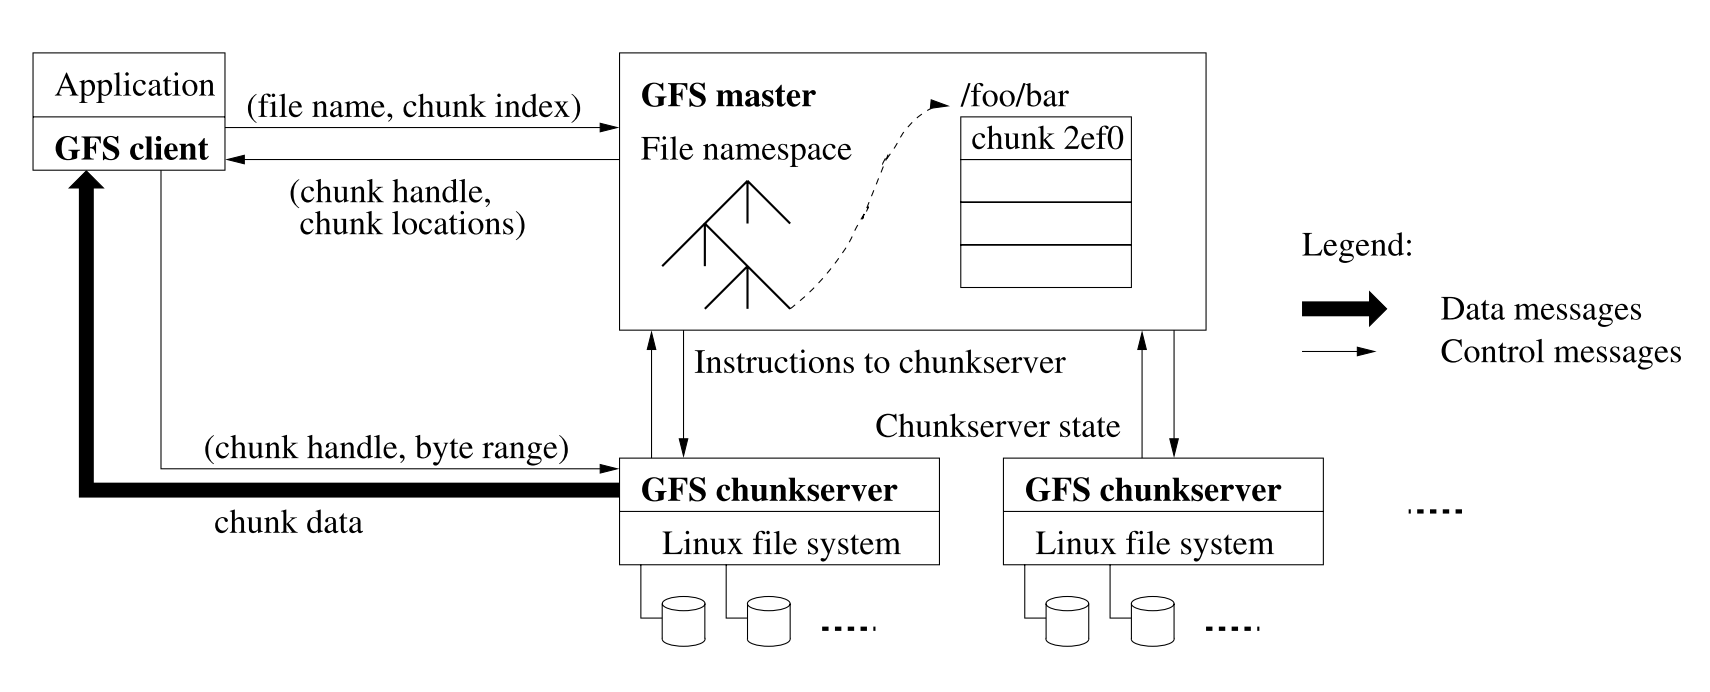
\includegraphics[width=0.95\textwidth]{image/gfs_architecture.png}
\caption{GFS architecture}
\label{fig:gfs_architecture}
\end{figure*}
%
The Google filesystem is the proprietary file system designed by 
Google~\cite{ghemawat2003google}.
%
It has a few impressive properties, such as the ability to reach a global
scalability~\cite{Ford2010a,Corbett2012a}, and the good performance on 
structured data~\cite{Chang2006a}.
%
However, publications are limited due to its proprietary nature. 
%
This section gives an overview of Google filesystem (GFS) based on the available
publications.

The initial design choices of GFS are explained by 
Ghemawat et al.~\cite{ghemawat2003google}.
%
It started from four observations regarding the unique usages and 
requirements by Google:
%
\begin{enumerate}
\item ``component failures are the norm rather than the exception";
\item ``files are huge by traditional standards";
\item ``most files are mutated by appending new data
		rather than overwriting existing data"; and
\item ``co-designing the applications and the file system API benefits the 
		overall system by increasing our flexibility."
\end{enumerate}
%
The extra flexibility as described by the fourth item enables GFS to 
make some radical design choices, for example, it does not comply to
any standard API.
%
In contrast, the other two surveyed filesystems both comply the 
standard API of POSIX.
%
We will revisit these observations and discuss how they
impact the design of GFS in the following discussion.


\subsubsection{Master-Server Architecture: Master}
GFS adopts a master-server architecture.
%
More specifically, each GFS cluster consists of one master node and 
multiple chunkservers; both are commodity machines.

The roles of master include:
\begin{enumerate}
\item maintaining all filesystem metadata, including
	namespace, access control, mapping from files to chunks, and current
	locations of chunks;
\item monitoring system state by sending periodical heartbeat messages and 
	collecting system state of individual chunkservers;
\item controlling system-wide activities, such as lease management, 
	garbage collection, chunk migrations; and
\item answering requests from clients.
\end{enumerate}

Because there is only one single master node in a GFS system, the master can
easily become a system bottleneck.
%
To prevent this from happening, the master takes a minimum involvement
in the fourth task: answering requests from clients.
%
More specifically, the master does not handle any of the actual file I/O
operations; rather, it sends instructions and re-directs actual file I/O 
operations to the proper chunkserver nodes.
%
These instructions include which chunkservers to look for, and what chunk 
handles to use.
%
Clients then interact with file chunkservers to finish the actual file I/O 
operations.


\subsubsection{Master-Server Architecture: Chunkserver}
The chunkservers in GFS are machines that actually stores data files.
%
Data is stored as chunks in GFS, so each chunkserver stores many data chunks.
%
The chunk size is an important parameter to tune the GFS, and 
64MB is decided to be a good balance between disk utilization and 
system performance.
%
%A file server always listens instructions from the master to perform 
%routine tasks, including:
A chunkserver always performs tasks from either instructions from the 
master, or the clients. 
%
Typically, these tasks include:
%
\begin{enumerate}
\item read and write operations per requests by clients;
\item maintenance tasks such as replicating an existing data chunk;
\item lease management, including requiring a lease, extending a lease, 
	and releasing a lease; and
\item rallying in a data flow along a chain of chunkservers. 
\end{enumerate}
%
We will discuss the last task in Section~\ref{}.

The overview of GFS architecture is shown in Figure~\ref{fig:gfs_architecture}.



\subsection{IBM GPFS: General Parallel File System}
\label{sec:archi_gpfs}
%
\begin{figure}
\centering
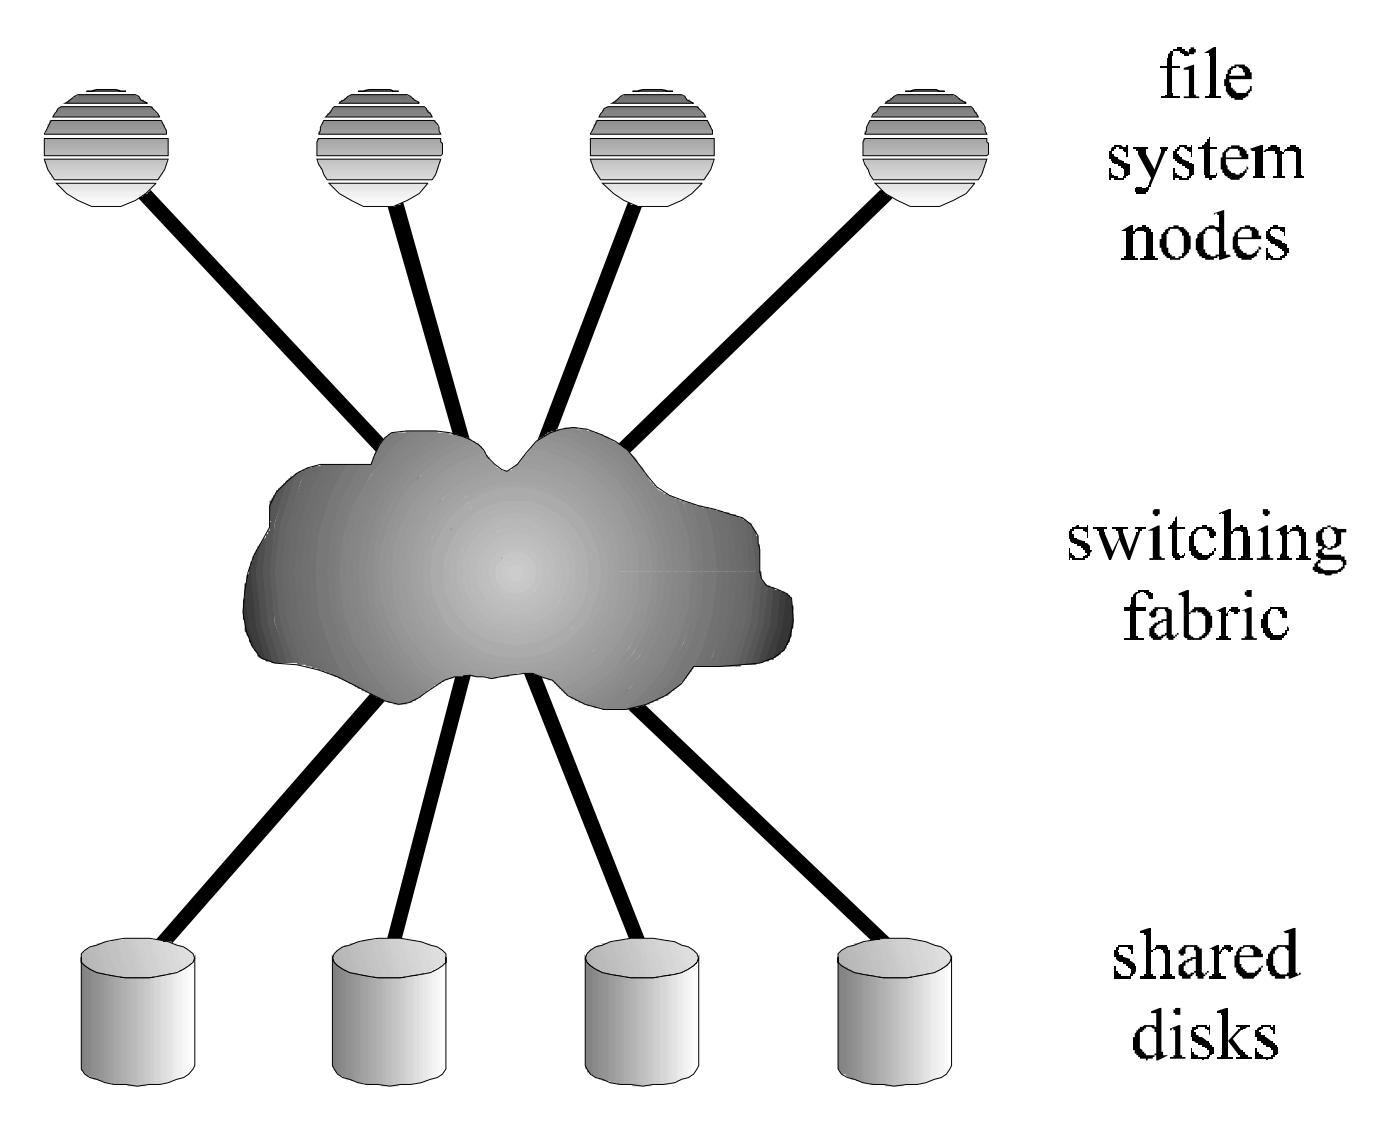
\includegraphics[width=0.95\columnwidth]{image/gpfs_architecture.png}
\caption{GPFS architecture}
\label{fig:gpfs_archi}
\end{figure}
%
The General Parallel File System (GPFS) from IBM is a popular filesystem
that is more widely adopted than the Google File System. 
%
In fact, it powers some of the most powerful supercomputers in the world,
including the third and fifth fastest supercomputers (Sequoia and Mira 
respectively) in the latest Top500 list~\cite{Strohmaier:2006:TS:1188455.1188474}.
%
Accordingly, there is more published research on GPFS than GFS.
%
However, because of the proprietary nature of GPFS, the publications on 
GPFS is also relatively limited. 
%
We provide an overview of the architecture of GPFS in this section.


\subsubsection{Decentralized Architecture}
GPFS adopts a decentralized architecture.
%
More specifically, there are cluster nodes and disks or disk subsystems.
%
Clusters and disks are connected over a switching fabric.
%
The architecture is decentralized in the sense that all cluster nodes 
have equal to the disks, and they provide equal functionalities and access
to user applications.

Data stored on GPFS is distributed into many stripes, and are essentially
placed on different disks.
%
This design enables parallel data access, which helps improving the overall
I/O performance.
%
We will discuss more about this parallel data access later in Section~\ref{}.

The locking mechanism of GPFS is mostly distributed as well with a few tasks
performed in a centralized fashion.
%
The centralized locking routines mainly takes care of updates on metadata
and configuration files.
%
Even these routines are centralized, the central coordinator is elected from
the pool of clusters, and can hardly run into a single-point failure problem.
%
Figure~\ref{fig:gpfs_archi} provides an overview of the GPFS architecture.



\subsection{Lustre File System}
\label{sec:archi_lustre}
%
\begin{figure}
\centering
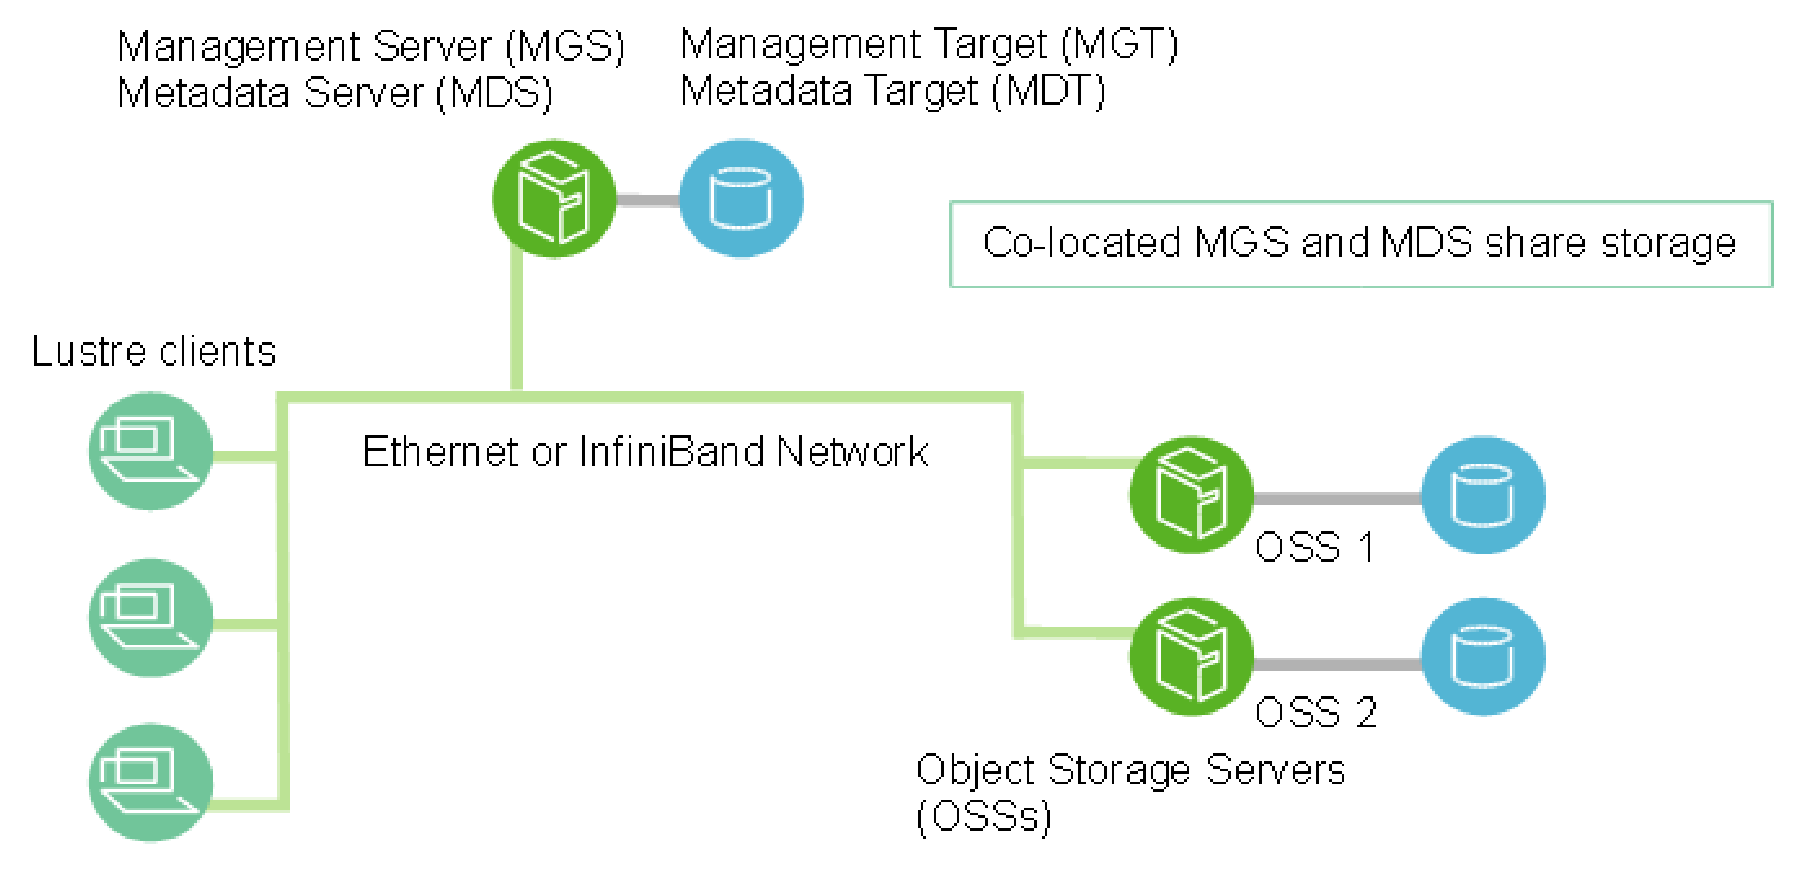
\includegraphics[width=0.99\columnwidth]{image/lustre_architecture.png}
\caption{Lustre architecture}
\label{fig:lustre_archi}
\end{figure}
%
Lustre is an open-sourced filesystem. 
%
Like GPFS, Lustre has also been used by many of the world's top supercomputers.
%
It is also the most intensively researched distributed file system among 
the three. 

\subsubsection{Lustre File System Architecture}
The Lustre file system has a similar architecture as GFS:
one node serves as management server (MGS); 
multiple object storage servers (OSS) actually stores data;
management server and object storage servers are connected via
high-speed network.
%
It should also be noted that later releases of Lustre do have support
for multiple metadata servers to provide better reliability.

On the management server side, it keeps all the metadata in object files,
named metadata target (MDT).
%
MDTs have information filenames, directories, permissions and file layout.
%
The MGS also provides network request handlings for local MDTs.

On the object storage server side, data is grouped as object storage targets
(OSTs). 
%
The mapping between OSSs and OSTs can be flexible, which means 
one OSS can have multiple OSTs, or
multiple OSSs have access to one OST, or
even a more complex $n$ to $m$ mapping.
%
The final choice of mapping scheme is based on the usage and the choice of 
hardware. 
%
For example, one OSS can host two OSTs to achieve redundency if using 
commodity storage, while utilize the complex $n$ to $m$ mapping to achieve
high performance if using enterprise-class storage arrays.
%
Figure~\ref{fig:lustre_archi} provides an overview of the Lustre architecture.


\subsection{Discussion on Three Architectures}
The three surveyed filesystems, GFS, GPFS, and Lustre represent two 
distinct architectures: architecture with a master node or 
architecture without a master node.
%
Both architectures have advantages and disadvantages.

GFS, Lustre have a master node, and this design has a major advantage
that it is easy to perform maintenance creating data replica; 
migrating partial data; detecting and 
from failures; communicating with clients; etc.
%
The master node has this advantage because it possesses a global knowledge
of the entire file system.
%
The disadvantage is also obvious that the master node can cause a 
single-point failure.
%
This disadvantage can be largely avoided by providing a replica of the master
node, as what Lustre does.
%
A less severe drawback is that the master node can become a system bottleneck.
%
Modern supercomputers tend to equip a large amount of memory and fast storage
such as solid state drives to tackle this problem.

GPFS uses a decentralized architecture without a master node.
%
This design has an obvious advantage that it has better tolerance on 
failure of single nodes.
%
This property is quite important on large scale systems.
%
The disadvantage of this decentralized architecture is that implementation
of many operations, like locks or leases, becomes complicated in many cases.
%






\section{Distributed File Partitions}
\label{sec:file_partition}
Distributed file systems provide a unified interface to applications and clients,
yet they consist of a number of disks and servers.
%
Partitioning files and put them on separate disks and servers is a common practice,
because this approach provides aggregated storage capacity and bandwidth.
%
This section surveys partitioning strategies adopted by the three file systems,
and disscuss the advantages and disadvantages of them.


\section{Achieve an Even Higher Performance}
\label{sec:performance}
We survey the efforts researchers have made to achieve an even better
performance on these three file systems.
%
The better performance here refers to characteristics such as throughput,
scalability, etc.


\subsection{GFS: Toward a Global Scalability}
\label{sec:gfs_scal}
%
\begin{figure}
\centering
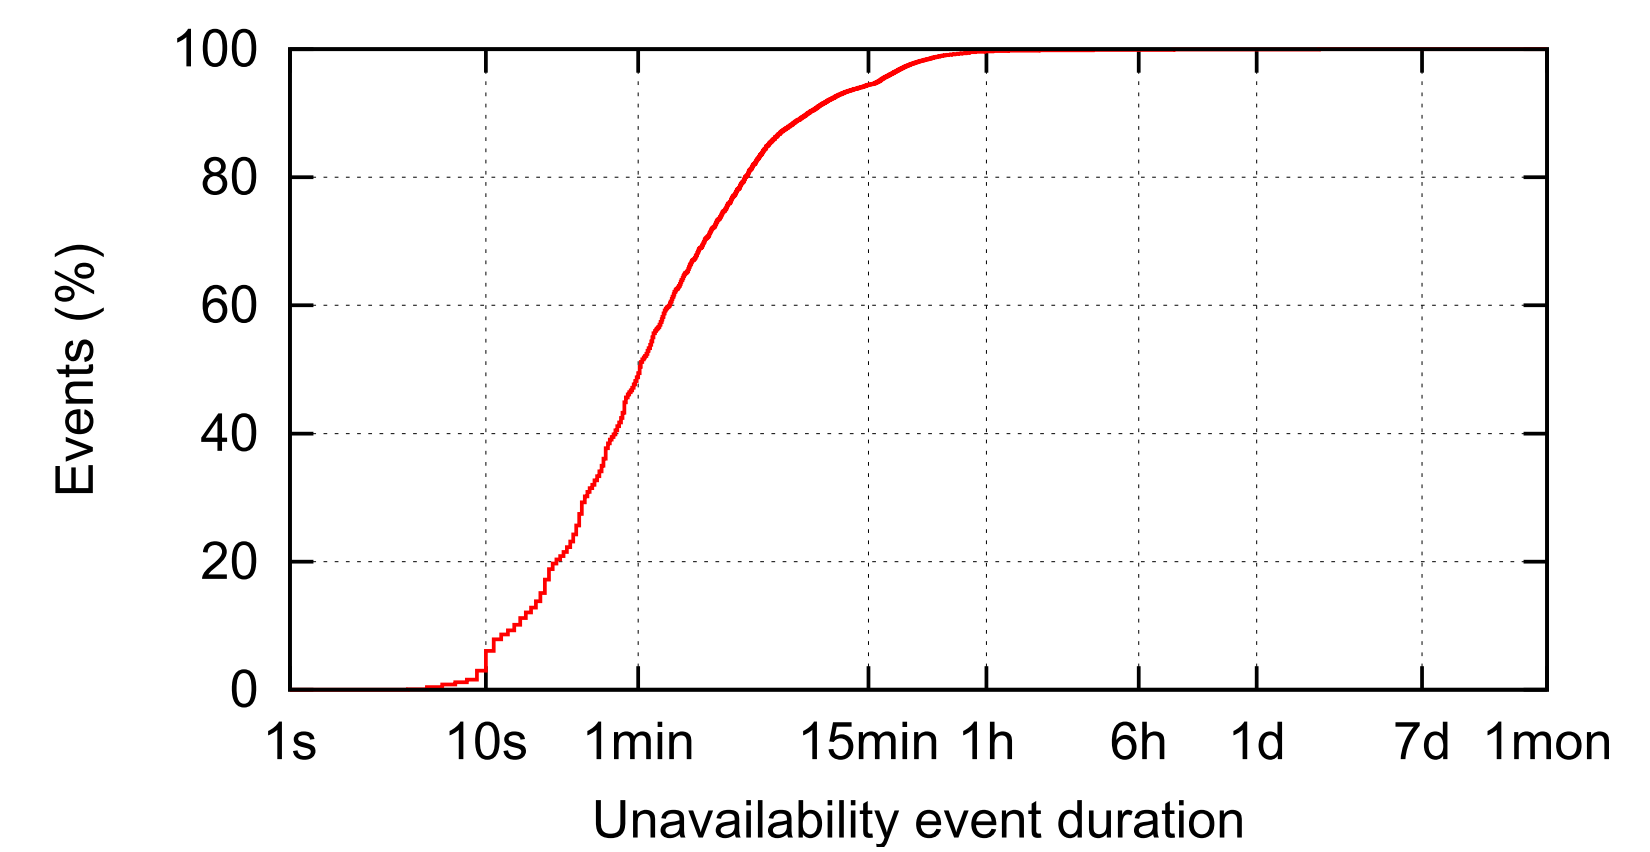
\includegraphics[width=0.99\columnwidth]{image/event.png}
\caption{Cumulative distribution function of the duration of node 
	unavailability periods.}
\label{fig:event}
\end{figure}
%
To achieve great scalability, a good handling of failures is necessary.
%
In the real application of GFS, many storage server nodes are called a cell.
%
A typical cell may comprise many thousands of nodes housed together in a 
single building or a set of co-located buildings.

To characterize the failures and availability of a GFS cell, we start from
the availability of single storage nodes.
%
A storage node becomes unavailable when it fails to respond positively 
to periodic health checking pings.
%
Nodes can become unavailable for a large number of
reasons. For example, a storage node or networking switch can be overloaded; 
a node binary or operating system may crash or restart; 
a machine may experience a hardware error; 
or the whole cluster could be brought down for maintenance. 
%
The vast majority of such unavailability events are transient and do not 
result in permanent data loss.
%
In fact, statistics show that less than 10\% of events last longer than 15 
minutes (see Figure~\ref{fig:event}).
%
For this reason, GFS typically waits 15 minutes before commencing 
recovery of data on unavailable nodes.

Two measurements are used to measure the stability of the GFS: 
average availability and mean time to failure (MTTF). 
%
Given a cluster of $N$ nodes, average availability is defined as following:
%
\begin{equation}
A_{N}=\frac{\sum_{N_i\in N} uptime(N_i)}{\sum_{N_i\in N}(uptime(N_i) + downtime(n_i))}
\end{equation},
%
where $uptime(N_i)$ and $downtime(N_I)$ refer to the length of time a node $N_i$
is available or unavailable.
%
MTTF is defined as following:
\begin{equation}
MTTF=\frac{uptime}{number of failures}.
\end{equation}


\subsubsection{Data Replication and Chunk Placement}
When a node failure causes the unavailability of a chunk within a stripe, 
we initiate a recovery operation for that chunk from the other available 
chunks remaining in the stripe.
%
Distributed file systems will necessarily employ
queues for recovery operations following node failure. 
These queues prioritize reconstruction of stripes which
have lost the most chunks.

To minimize the effect of large failure bursts in a single failure domain,
we also consider a rack-aware policy.
%
A rack-aware policy is one that ensures that no two chunks in a stripe are 
placed on nodes in the same rack.
%
Research has shown that using a rack-aware placement policy increases 
the stripe MTTF by a factor of 3 typically.

The researchers also used a Markov model to validate some findings.
%
Two interesting finds are:
\begin{enumerate}
\item improvements of component failure rates below the node layer
	of the storage stack do not significantly improve data availability.
	For example, a 10\% reduction in the disk failure rate increases 
	stripe availability by less than 1.5\%. On the other hand, cutting node 
	failure rates by 10\% can increase data availability by 18\%. 
\item Replicating data across multiple cells  greatly improves availability 
	because it protects against correlated failures.
	It also greatly increase the inter-cell bandwidth requirement, so there 
	is still trade-offs to make.
\end{enumerate}


\subsubsection{Google Services Built on Top of the GFS}
Because of the extreme scalability of GFS, other services become available
on top of the GFS.
%
Corbett et al.~\cite{Corbett2012a} demonstrated a database system in in Google.
%
It is the first system to distribute data at global scale and support 
externally-consistent distributed transactions. 
%
Chang et al.~\cite{Chang2006a} demonstrated Bigtable, 
a distributed storage system for managing structured data.
%
It is able to scale to a very large size: petabytes of data across thousands of commodity servers.
%
Even though many Google applications place diverse demands on Bigtable, 
Bigtable is still able to provide high-performance solutions for all these
services.



\subsection{GPFS to Achieve Better Performance}
GPFS has demonstrated great performance in high scalability, 
fast scan, and high throughput.
%
There are many research of GPFS on real systems, for example,
Yu et al.~\cite{Yu2006} demonstrated a highly scalable GPFS file system
with satisfactory overall performance;
%
Andrews et al.~\cite{Andrews2005} researched from both theoretical 
and practical sides of the performance of GPFS file system
in an inter-state scale.
%
Further, Freitas et al.~\cite{freitas2011gpfs} reported performance 
of GPFS file system to scan 10 billion files in 43 minutes. 
%
We elaborate these results in the following subsections.

\subsubsection{GPFS to achieve global scalability}
%
\begin{figure}
\centering
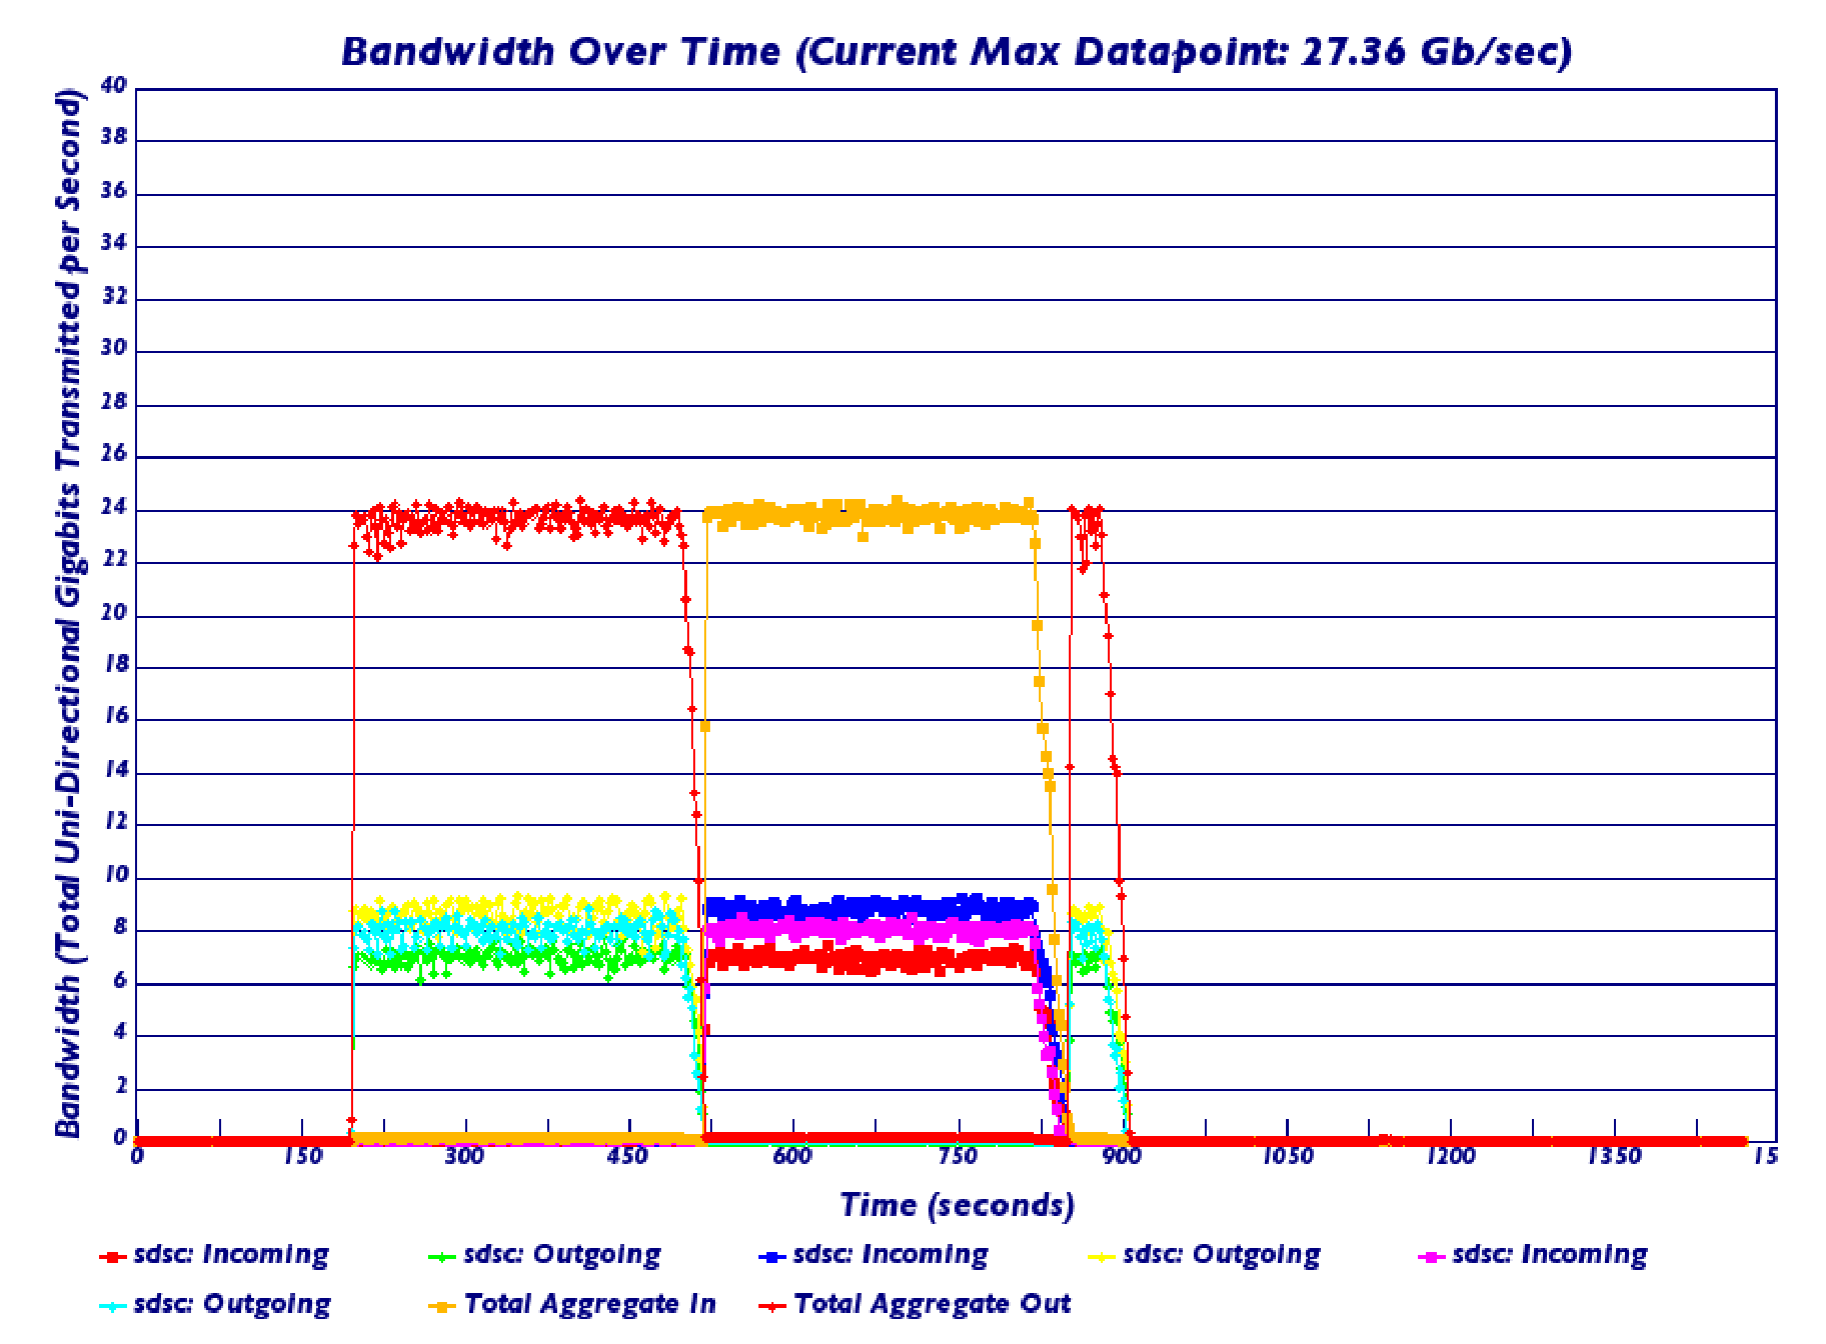
\includegraphics[width=0.99\columnwidth]{image/sc04.png}
\caption{Measured WAN performance at SC'04 for sequential reads and writes.}
\label{fig:sc04}
\end{figure}
%
Andrews et al.~\cite{Andrews2005} have demonstrated the high scalability 
of the GPFS file system in two consecutive SuperComputing (SC) conferences.
%
In these demonstrations, data centers across the US continent are connected
using the GPFS file system.
%
These data centers include: San Diego Supercomputing Center (SDSC) in San
Diego, CA,
the National Center for Supercomputing Applications (NCSA) in 
Urbana, IL, 
and the conference location in Phoenix, AZ and Pittsburgh, PA.
%
In the SC'03 conference, the researchers used a 10Gb/s connection at the 
conference center, and the GPFS achieves around 9Gb/s read/write speed working on 
storage in San Diego.
%
This is about 90\% percent of the connection bandwidth.
%
In the SC'04 conference, the researchers used a 40Gb/s connection at the 
conference center, with GPFS file system connecting to storage in both 
SDSC and NCSA sites.
%
They achieved around 27Gb/s sustaining speed, which is about 67\% of the 
connection bandwidth. 
%
Figure~\ref{fig:sc04} plots the bandwidth overtime in this test.
%
Given the large physical distance (from the west coast to the east coast)
of these experiments, GPFS has demonstrated great scalability.



\subsubsection{GPFS to Achieve Fast Scan}
Distributed file systems are good at providing big throughput, but are traditionally
bad at operations on many small files.
%
Freitas et al.~\cite{freitas2011gpfs} experimented the use of solid state drives
(SSDs) to store the metadata of a file system, and reported satisfactory
result on scanning 10 billion files on a GPFS file system.
%
It took 43 minutes in this test.

The scan over 10 billion files takes 2 steps.
%
In the first step, it parallelly traverses all directories. 
%
Each processor takes care of a sub-tree.
%
When this phase is complete, the full path to every file and that file’s inode number is stored in a series of temporary files.
%
The second step is sequential scan.
%
It begins by assigning the temporary files to the processes running on each node.
%
Each set of temporary files contains a range of inodes in the file system.
%
The files’ inodes are read directly from disk via a GPFS API, thus providing 
the files’ attributes such as owner, file size, atime and it includes 
the files’ extended attributes.
%
Figure~\ref{fig:gpfs_scan} shows the number of reads per second in this test.
%
\begin{figure}
\centering
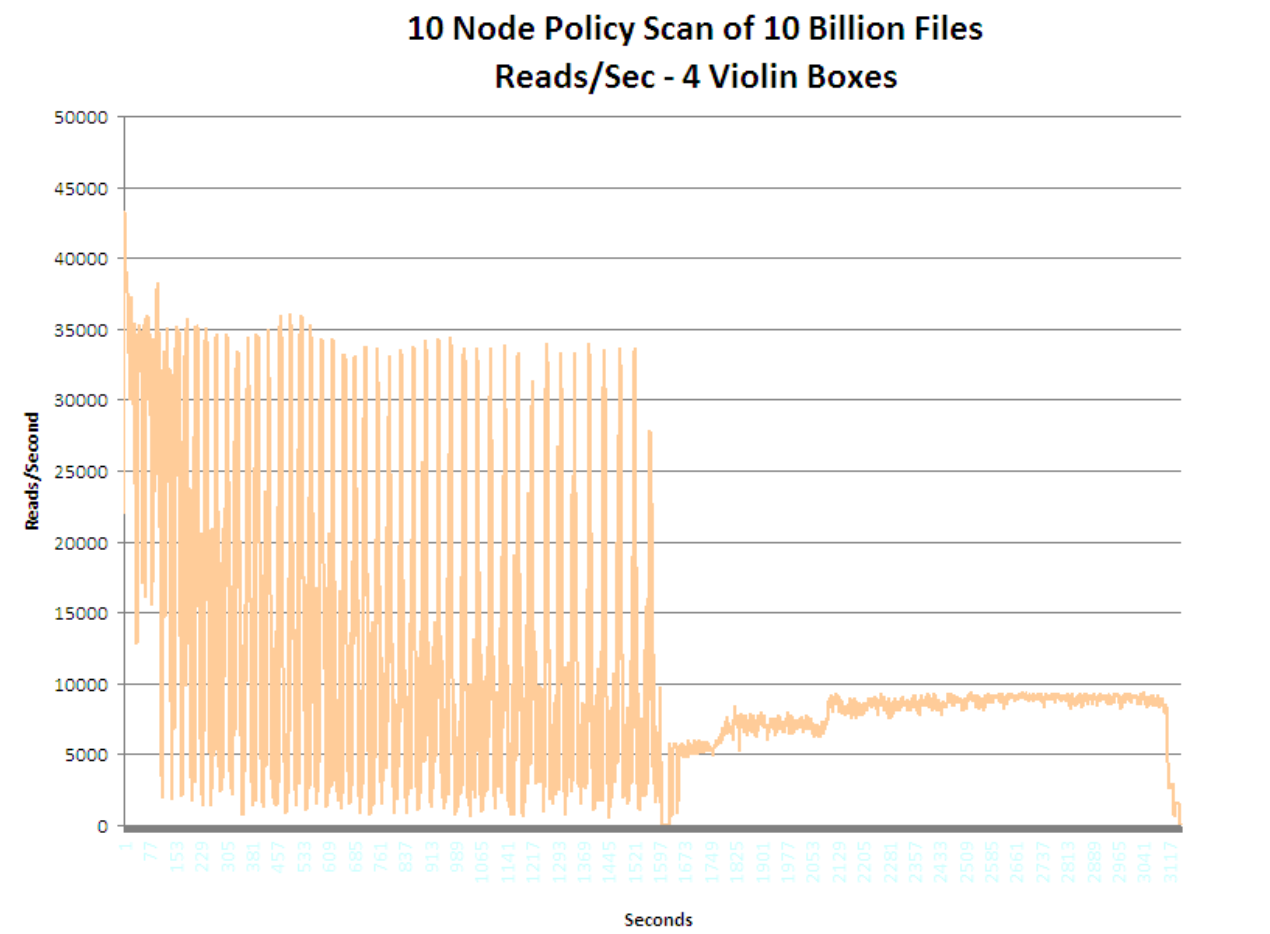
\includegraphics[width=0.99\columnwidth]{image/gpfs_scan.png}
\caption{Aggregate read operations per second.}
\label{fig:gpfs_scan}
\end{figure}

The first step takes about 20 minutes. 
%
This step is highly input operations intensive, because it reads many random
locations in the file system.
%
This step of scan greatly benefits from the underlying SSD storage that keeps 
all the metadata.
%
The second step takes about 23 minutes.
%
It reads the temporary files created by the first phase. 
%
It is essentially bandwidth bound.


\subsubsection{GPFS to Achieve High Bandwidth}
%
\begin{figure}
\centering
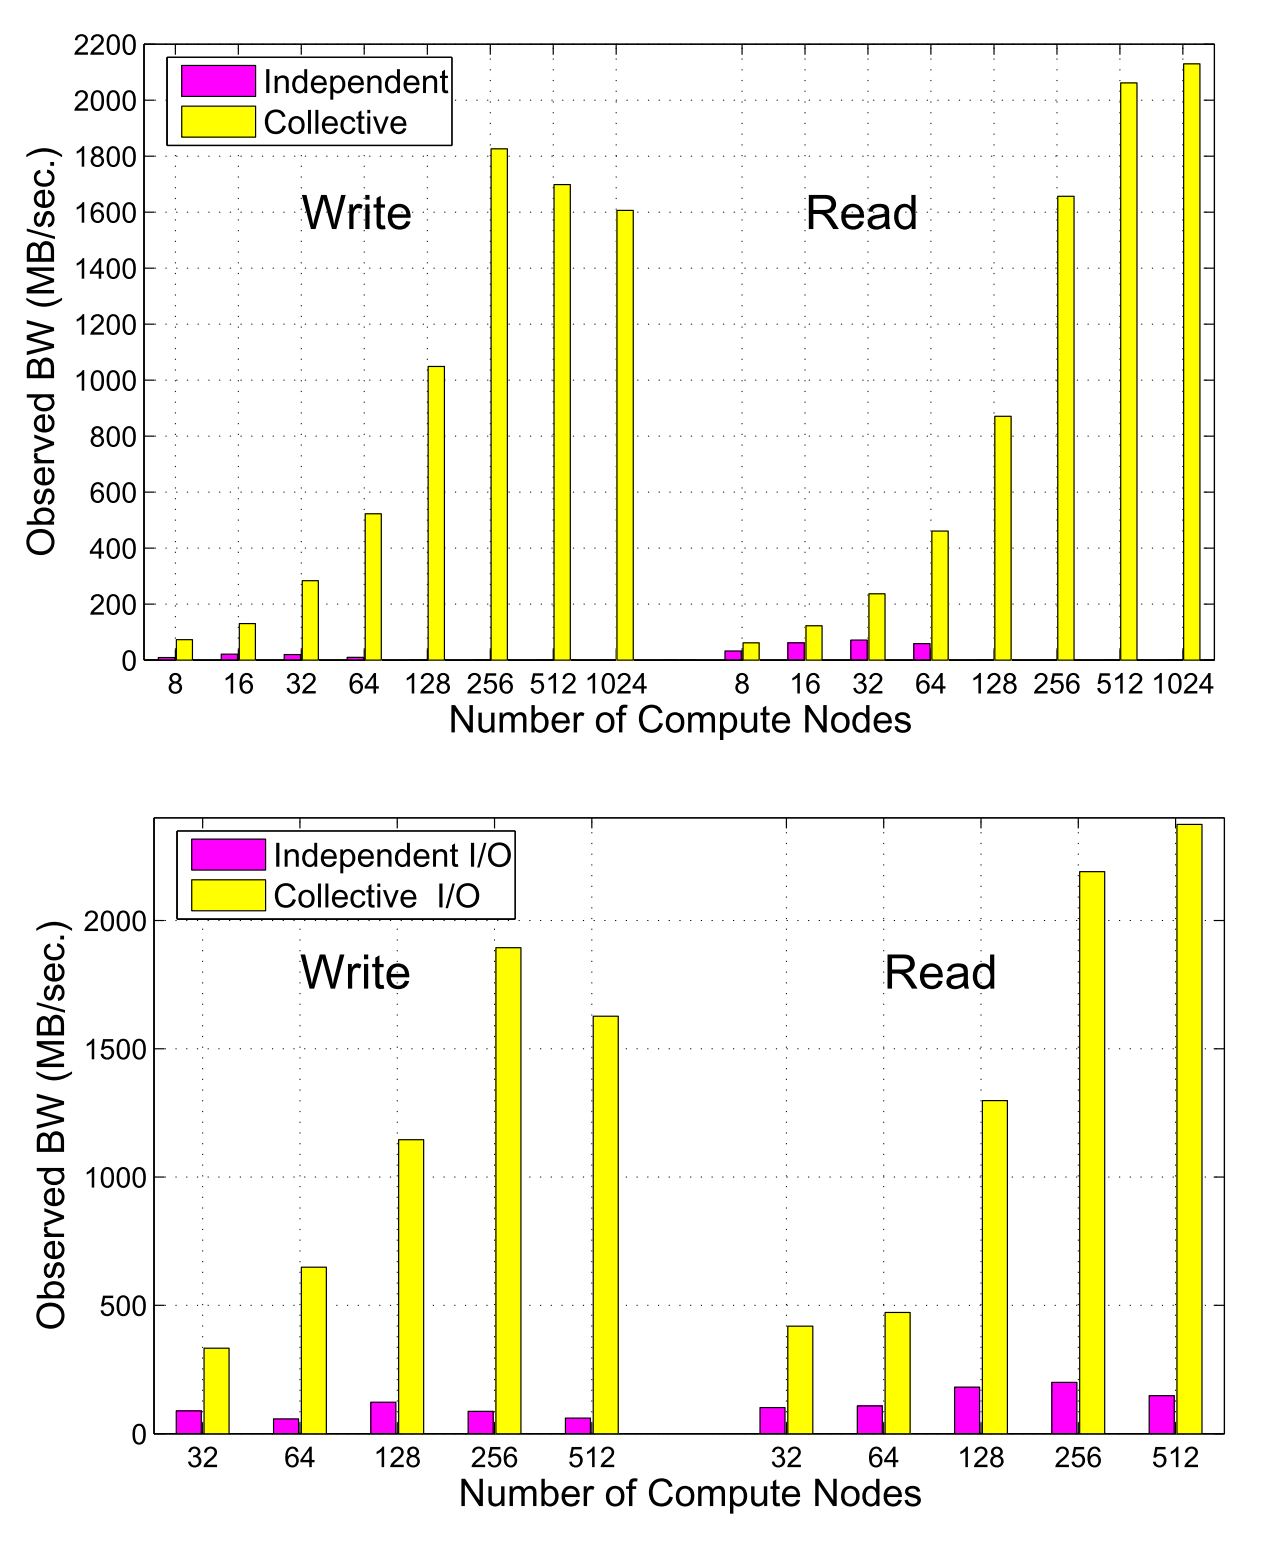
\includegraphics[width=0.99\columnwidth]{image/bw.png}
\caption{Improvement on bandwidth of GPFS file system after applying collective I/O.}
\label{fig:bw}
\end{figure}
%
Ross et al.~\cite{Yu2006} used MPI I/O on top of GPFS to achieve good read/write
performance on an IBM Blue Gene supercomputer.
%
They used the ROMIO MPI implementation, and tuned it to work best with GPFS.
%
For example, they implemented collective buffering in MPI I/O, which 
rearranges and aggregates data in memory prior to writing to files to 
reduce the number of disk accesses.
%
For scientific applications, collective buffering is effective for 
achieving scalable I/O.
%
They also replaced a few MPI implementations based on the characteristics
of the GPFS system.
%
For example, they replaced the use of the point-to-point functions with 
MPI\_Alltoallv, which can utilize up to 98\% of the peak bandwidth within 
a compute node.
%
They also replaced the MPI\_Allgather with an MPI\_Allreduce, 
which performs much better for short and medium sized messages. 
%
The results show that the achieved bandwidth with collective I/O is 
significantly improved, as shown in Figure~\ref{fig:bw}.



\subsection{Higher Performance on Lustre File System}
%
The Lustre file system receives most intensive research because of its
open source nature. 
%
%Here is a selected collection and the main topic of each paper:
For example, Crosby~\cite{Crosby2009} characterized the performance of 
Lustre file system on a real supercomputer system;
%
Xie et al.~\cite{Xie2012} specifically characterized output performance
with respect to a number of system parameters;
%
Schwan~\cite{Schwan2003} and Henschel et al.~\cite{Henschel2012} 
demonstrate implementations of Lustre to achieve the best performance
on real systems; 
%
Lofstead et al.~\cite{lofstead2010managing} specifically researched 
interference effects measured on two real systems; and
%
Shipman et al.~\cite{Shipman2010} summarized real lessons learned 
to achieve high performance on a very large scale Lustre file system.

To focus our discussion on the core performance issues, 
this subsection first identifies a few parameters that affect the performance
of Lustre file system in a real production environment, and then provides
a few demonstrations of Lustre file system to achieve both high scalability
and performance. 


\subsubsection{Performance Characteristics of the Lustre File System}
%
\begin{figure}
\centering
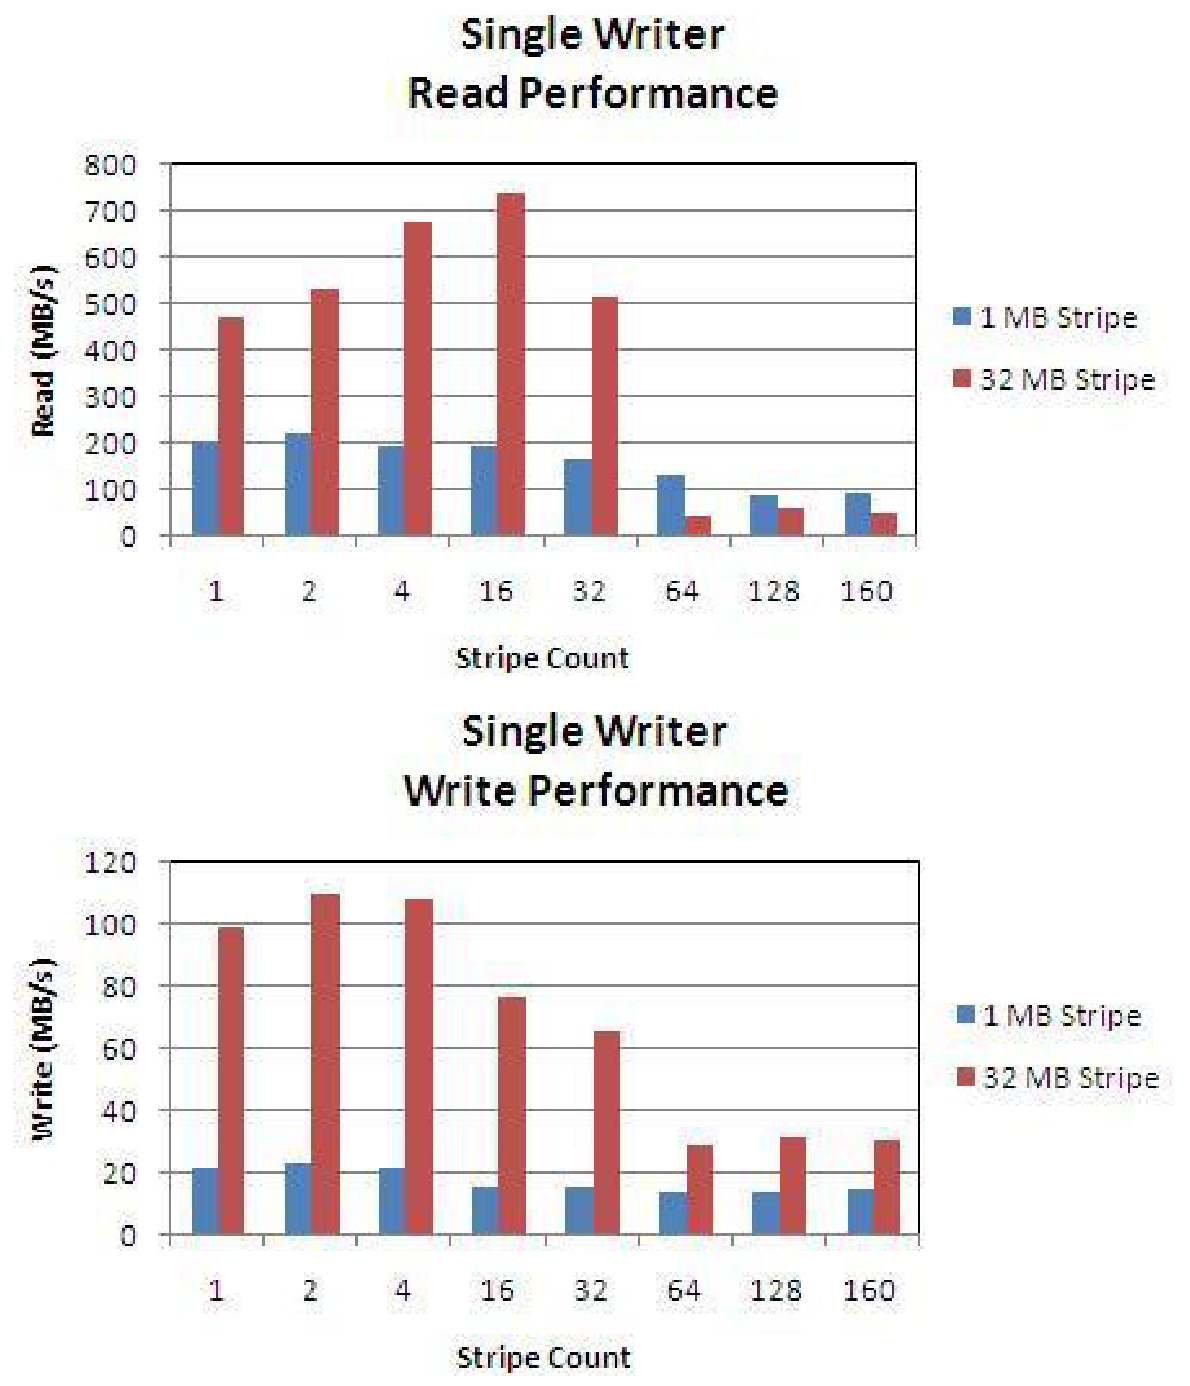
\includegraphics[width=0.99\columnwidth]{image/lustre_rw.png}
\caption{Read and write performance of Luster file system on a real system
	as a function of stripe count.}
\label{fig:lustre_rw}
\end{figure}
%
Crosby et al.~\cite{Crosby2009} characterized the performance of Lustre 
file system on a real system: a Cray XT5 supercomputer at the Oak Ridge
National Lab.
%
Striping is an important mechanism in Lustre to achieve high 
throughput~\ref{sec:stripe_Lustre}, so it is important to test the I/O
performance as a function of the stripe sizes.
%
The researchers performed read and write tests on data files with size
varying from 32MB to 5GB on the real system, and plotted their performance
as shown in Figure~\ref{fig:lustre_rw}.
%
It shows that both write and read performance significantly degrades when
the stripe count is greater than 32, with 16 or 4 probably being the 
sweet spot.
%
These tests also show that a larger sized stripe, for example 32MB other than 
1MB, is helpful to achieve a better performance.


\subsubsection{High Scalability of Luster File System}
%
\begin{figure*}
\centering
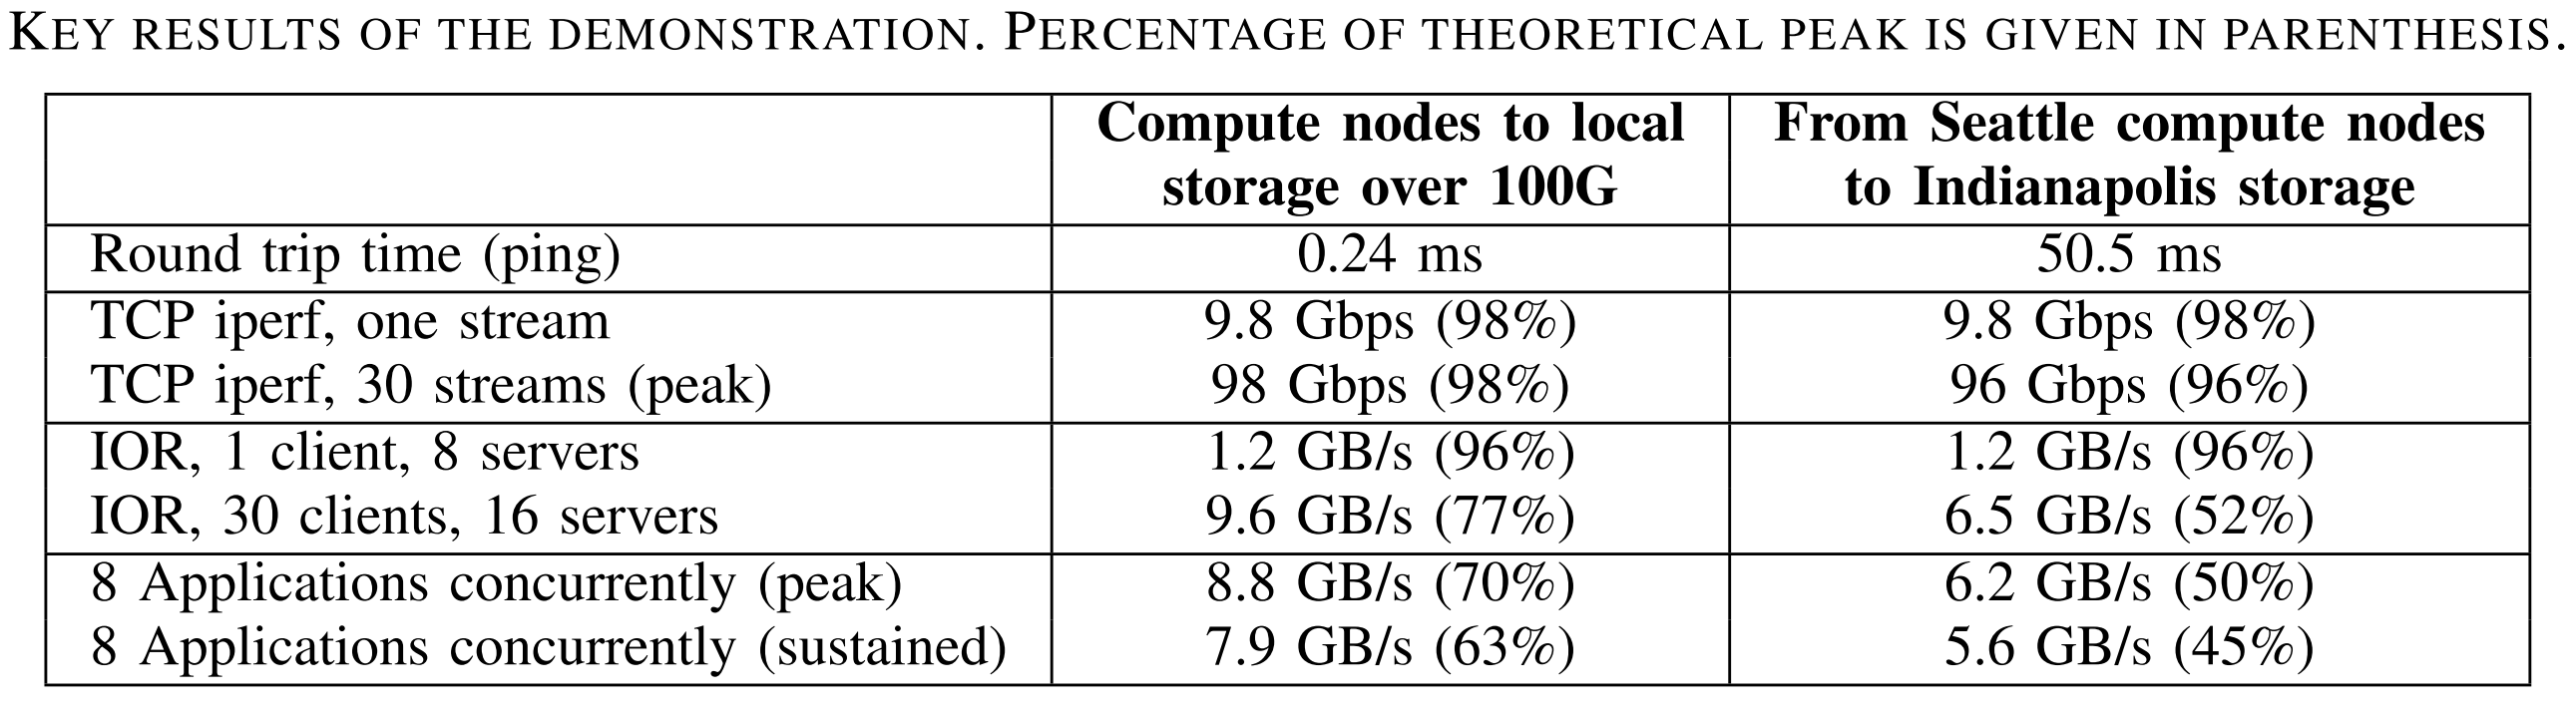
\includegraphics[width=0.9\textwidth]{image/lustre_scale.png}
\caption{Scalability test of Lustre File System. This test compares the same
	software and hardware performing either on the local site, or through a 
	WAN connection.}
\label{fig:lustre_scale}
\end{figure*}
%
Researchers have also investigated the capability of Lustre file system
to achieve a great scalability.
%
Henschel et al.~\cite{Henschel2012} demonstrated a Lustre file system over
a 100Gbps wide area network of 3,500km.
%
These researchers compared the same setups of hardware and software on a local
machine room, as well as spanning from Seattle to Indianapolis.
%
Evaluations are performed on both benchmark test suits as well as real-world
applications.
%
The results are shown in Figure~\ref{fig:lustre_scale}.

These evaluations show a 20\% to 30\% degradation of throughput 
when the file system is set to cross the country.
%
This result is satisfactory considering the many technical difficulties 
associated with a WAN and the complexity of a distributed file system.
%
These results serve as a concept demonstration that a Lustre file system
with very big scales is possible.














\section{Conclusion}
This paper surveys performance factors of three popular distributed 
file systems: the Google File System (GFS), IBM General Parallel 
File System (GPFS), and Lustre File System.
%
We especially focused on the 1) different architecture design,
2) file partitioning scheme, and 3) efforts and demonstrations to achieve
higher performance using these three file systems.
%
Architecture wise, both GFS and Lustre adopt a master-server mode, whereas
GPFS adopts a decentralized architecture.
%
File partition scheme is more similar among these three file systems, 
with a different in the choice of chunk size.
%
Higher performance is achieved by all three file systems, including 
high robust to failures, high throughput, and high scalability to span
thousands of miles.

%\section{Briefs}
%\label{sec:brief}
%%The following papers characterize behaviors of distributed file systems
%on supercomputers:
%\cite{Xie2012}, \cite{Henschel2012}, \cite{Crosby2009}, \cite{Borrill2009}.

%The following papers discuss approaches to better work with distributed 
%file systems given the characters above:
%\cite{Shipman2010}, \cite{Yu2006}, \cite{Tian2011}, \cite{Lofstead2010},
%\cite{Lofstead2009}.

\subsection{Research on Lustre}
Many research papers have focused on the performance issue of 
Lustre file systems. 
%
Here is a selected collection and the main topic of each paper:
Crosby~\cite{Crosby2009} characterized the performance of Lustre file system
on a real supercomputer system;
%
Xie et al.~\cite{Xie2012} specifically characterized output performance
with respect to a number of system parameters;
%
Schwan~\cite{Schwan2003} and Henschel et al.~\cite{Henschel2012} 
demonstrate implementations of Lustre to achieve the best performance
on real systems; 
%
Lofstead~\cite{lofstead2010managing} et al. specifically researched interference effects
measured on two real systems; and
%
Shipman et al.~\cite{Shipman2010} summarized real lessons learned 
to achieve high performance on a very large scale Lustre file system.


\subsection{Research on GPFS}
GPFS comes with most IBM supercomputers, and also receives intense study
in terms of its performance.
%
Yu et al.~\cite{Yu2006} demonstrated a highly scalable GPFS file system
with satisfactory overall performance;
%
Andrews et al.~\cite{Andrews2005} researched from both theoratical 
and practical sides of the performance of GPFS file system
in an inter-state scale.
%
Further, Freitas et al.~\cite{freitas2011gpfs} reported performance 
of GPFS file system to scan 10 billion files in 43 minutes. 


\subsection{Research on Google File System}
Even Google intends to keep the Google File System restrict
to its own use, it still publishes a few papers discussing the 
performance of Google File System.
%
In addition to the original paper that specifies the design of
Google File System~\cite{ghemawat2003google},
Chang et al.~\cite{Chang2006a} also discusses efforts to make Google
File System better handle structured data;
Ford et al.~\cite{Ford2010a} and Corbett et al.~\cite{Corbett2012a}
also disscussed how Google File System achieves a global scalability.


The rest of this survey paper will elaborate above mentioned studies 
to provide a big picture on performance issues of parallel file systems
and available approaches to best make use of these systems.


%% file citations.bib contains all the biblography
\bibliography{main}
\end{document}
